\section{Introduction (2~p)}\label{sec:introduction}

\footnote{The authors acknowledge support by the state of Baden-Württemberg through \href{https://www.bwhpc.de/}{bwHPC}.}
\newpage

\section{Related Work (3~p)}\label{sec:related-work}

\textbf{Trade Classification in Option Markets}

While classical trade classification algorithms are extensively tested in the stock markets (e.g., \textcite{chakrabartyTradeClassificationAlgorithms2012}; \textcite{odders-whiteOccurrenceConsequencesInaccurate2000}), few works have examined trade classification in option markets.

\textcite[882--883]{savickasInferringDirectionOption2003} are the first to compare the tick rule, quote rule, the Lee and Ready algorithm and the \cgls{EMO} rule for options traded at the \cgls{CBOE}. The data set spans a period from July 3, 1995 -- December 31, 1995 consisting of $869{,}217$ matched trades. The authors report the highest accuracies for the quote rule (\SI{78.98}{\percent}) and find that all rules perform worst when applied to index options. In general, the trade classification rules exhibit significantly lower classification accuracies on options data than with stock data, urging the need for improved classifiers.

The most exhaustive study is the one of \textcite[1--39]{grauerOptionTradeClassification2022}.  The authors test the accuracy of the classical quote rule and tick rule, and hybrids thereof on two large-scale data sets spanning a period from 2005 - 2017. Consistently for options traded at the \cgls{ISE}, and \cgls{CBOE} classical rules like the popular Lee and Ready algorithm only achieve accuracies of \SI{62.53}{\percent} or \SI{62.03}{\percent} and are thus significantly smaller than in the stock market. In line with the research of  \textcite[886]{savickasInferringDirectionOption2003}, the reported accuracies are inversely proportional to the rule's reliance on past transaction prices. In particular, the tick rule performs worst with accuracies marginally different from a random guess. Overall, the reported success rates deteriorate between both studies and over time. As a remedy, \textcite[14--17]{grauerOptionTradeClassification2022} introduce two additional rules based on the trade and quote sizes. The \textit{depth rule} is an alternative to the tick rule for classifying midspread trades in the Lee and Ready algorithm and \cgls{EMO} rule. It assigns the aggressor of the trade based on the depth at the bid or ask. Together with the \textit{trade size rule}, their second rule, which classifies trades with a trade size matching the size of the bid or ask quote, can substantially improve the performance of classical algorithms. The ensemble of rules achieves an accuracy between \SI{73}{\percent} and \SI{75}{\percent} surpassing primary rules by more than \SI{10}{\percent}, at the cost of data efficiency.

The work of \textcite[1--39]{grauerOptionTradeClassification2022} is important in two ways. First, the data set is identical to ours, which enables a fair comparison between classical rules and machine learning-based predictors. Second, their stacked combinations of the trade size rule, depth rule, and common trade classification algorithms achieve state-of-the-art performance in option trade classification and are thus a rigorous benchmark.

\textbf{Trade classification using machine learning}

\textcite[5]{rosenthalModelingTradeDirection2012} bridges the gap between classical trade classification and machine learning by fitting a logistic regression model on lagged and unlagged predictors inherent to the tick rule, quote rule, and \cgls{EMO} algorithm, as well as a sector-specific and a time-specific term. Instead of using the rule's discretized outcome as a feature, \textcite[481--482]{rosenthalModelingTradeDirection2012} models the rules through so-called information strength functions. The proximity to the quotes, central to the \cgls{EMO} algorithm, is thus modelled by a proximity function. Likewise, the information strength of the quote and tick rule is estimated as the log return between the trade price and the midpoint or the previous trade price. However, it only improves the accuracy of the \cgls{EMO} algorithm by a marginal \SI{2}{\percent} for Nasdaq stocks and \SI{1.1}{\percent} for \cgls{NYSE} stocks \textcite[15]{rosenthalModelingTradeDirection2012}. Our work aims to improve the model by exploring non-linear estimators and minimizing data modelling assumptions.

The work of \textcite[483]{blazejewskiLocalNonParametricModel2005} compares a $k$-nearest neighbour classifier against logistic regression, as well as simple heuristics like the majority vote over past trades for signing trades at the Australian stock exchange. Their results indicate that the parametric $k$-nearest neighbour classifier improves upon a linear logistic regression in terms of classification accuracy, even when trained on fewer features. The work is unique from the remaining works about feature set definition. Notably, \textcite[3]{blazejewskiLocalNonParametricModel2005} use no quote or trade prices, but rather the order book volumes, trade sizes, and past trade signs for classification. No accuracies for classical trade signing rules are reported, which impedes a comparison across different works. In line with their results, we focus on non-linear models in the form of gradient boosting and transformers. Additionally, our paper addresses the mentioned shortcomings by benchmarking against state-of-the-art trade classification rules. We share the idea of using the trade size, as well as the bid and ask sizes for classification for some of our feature sets, but greedily predict using non-historic features.

Closest to our work is a publication of \textcite[1--58]{ronenMachineLearningTrade2022}. Therein, the authors compare a selection of machine learning algorithms against classical trade signing rules in the bond and stock market. Their comparison is the first to consider logistic regression, a random forest, as well as \glspl{feed-forward-network}. Over a wide range of feature sets the tree-based ensemble consistently outperforms by out-of-sample accuracy the tick rule and Lee and Ready algorithm, as well as all remaining machine learning models. For the TRACE and ITCH data set, their best variant of the random forest outperforms the tick rule by \SI{8.3}{\percent} and \SI{3.3}{\percent}, respectively \autocite[57]{ronenMachineLearningTrade2022}. Whilst the superiority of random forests is consistent for the bond and equity market, fitted classifiers do not transfer across markets, as diminishing accuracies for the transfer learning by model transfer indicate.

The results convincingly demonstrate the potential of machine learning, i.e., of tree-based ensembles, for trade classification. Yet, the comparability of the results is limited by the classifier's reliance on additional features beyond quote and price data. Albeit, \textcite[4]{ronenMachineLearningTrade2022} consider a wide range of approaches, their selection leaves the latest advancements in artificial neural networks and ensemble learning aside and is mainly guided by computational constraints. Even if the focus is on standard techniques, the unclear research agenda concerning model selection, tuning, and testing hampers the transferability of their results to the yet unstudied option market.

In summary, machine learning has been applied successfully in the context of trade classification. To the best of our knowledge, no previous work perform machine learning-based classification in the options markets.

\newpage
\section{Rule-Based Approaches}\label{sec:rule-based-approaches} 

Every option trade has a buyer and seller side. For a plethora of problems in option research, it's also vital to determine the party that initiated the transaction. The trade initiator is binary and can either be the seller or the buyer. Consequently, we denote it by $\gls{y} \in \{0,1\}$, whereby $y=0$ indicates a seller-initiated and $y=1$ a buyer-initiated trade. As the trade initiator is commonly not provided with the option data sets, it must be inferred using trade classification algorithms \autocite[][453]{easleyOptionVolumeStock1998}.

The following section introduces basic rules for option trade classification. We start with the classical quote and tick rule and continue with the more recent depth and trade size rule. Our focus is on classification rules, that sign trades on a trade-by-trade basis. Consequently, we omit classification rules for aggregated trades, like the \cgls{BVC} algorithm of \textcite[][1466--1468]{easleyFlowToxicityLiquidity2012}.

\subsection{Basic Rules}\label{sec:basic-rules}

This chapter presents foundational classification rules, that may be used for trade classification as-is or integrated into a hybrid algorithm.

\subsubsection{Quote Rule}\label{sec:quote-rule}

The quote rule classifies a trade by comparing the trade price against the corresponding quotes at the time of the trade. We denote the sequence of trade prices of the $i$-th security at time $t$ by $p_{i,t}$ and the contemporaneous ask by $a_{i,t}$ and bid by $b_{i,t}$. If the trade price is above the midpoint of the bid-ask spread, denoted by $m_{i,t} = \tfrac{1}{2}(b_{i,t} + a_{i,t})$, the trade is classified as a buy and if it is below the midpoint, as a sell \autocite[][41]{harrisDayEndTransactionPrice1989}. Thus, the classification rule on $D = \left\{(p_{i,t}, m_{i,t}) \in \mathbb{R}^2: p_{i,t} \neq m_{i,t}\right\}$ is given by:

\begin{equation}
  \operatorname{quote}\colon D \to \left\{0, 1\right\},\quad
  \operatorname{quote}(p_{i,t}, m_{i,t})=
  \begin{cases}
    0, & \text{if}\ p_{i, t}>m_{i, t}  \\
    1, & \text{if}\ p_{i, t}<m_{i, t}. \\
  \end{cases}
\end{equation}

By definition, the quote rule cannot classify trades at the midpoint of the quoted spread. \textcite[][241]{hasbrouckTradesQuotesInventories1988} discusses multiple alternatives for signing midspread trades including ones based on the subsequent quotes, and contemporaneous, or the subsequent transaction. Yet, the most common approach to overcome this limitation is, to couple the quote rule with other approaches, as done in \cref{sec:hybrid-rules}

The quote rule requires matching one bid and ask quote with each trade based on a timestamp. Due to the finite resolution of the dataset's timestamps and active markets, multiple quote changes can co-occur at the time of the trade, some of which, may logically be after the trade. As such, it remains unclear which quote to consider in trade classification, and a quote timing technique must be employed. Empirically, the most common choice is to use the last quote in the order of the time increment (e.g., second) before the trade \autocite[][1765]{holdenLiquidityMeasurementProblems2014}.

The quote rule requires both price and quote data, which affects the data efficiency. The reduced dependence on past transaction prices and the focus on quotes has nonetheless positively impacted classification accuracies in option markets, as studies of \textcite[][886]{savickasInferringDirectionOption2003} and \textcite[][3]{grauerOptionTradeClassification2022} reveal. Especially, if trade classification is performed on the \cgls{NBBO}.


\subsubsection{Tick Test}\label{sec:tick-test}

A common alternative to the quote rule is the tick test. Based on the rationale that buys increase the trade price and sells lower them, the tick test classifies trades by the change in trade price \autocite[][271]{easleyDiscerningInformationTrade2016}. It was first applied in \textcites[][244]{holthausenEffectLargeBlock1987}[][240]{hasbrouckTradesQuotesInventories1988}.

The tick test, $\operatorname{tick}\colon \mathbb{R}^2 \to \left\{0,1\right\}$, is defined as:

\begin{equation}
  \operatorname{tick}(p_{i, t-1}, p_{i,t})=
  \begin{cases}
    1,                                         & \text{if}\ p_{i, t} > p_{i, t-1} \\
    0,                                         & \text{if}\ p_{i, t} < p_{i, t-1} \\
    \operatorname{tick}(p_{i,t-2}, p_{i,t}), & \text{else}.
  \end{cases}
  \label{eq:tick-test}
\end{equation}


Considering the cases in \cref{eq:tick-test} the trade price is higher than the previous price (uptick) the trade is classified as a buy. Reversely, if it is below the previous price (downtick), the trade is classified as a sell. If the price change is zero (zero tick), the signing uses the last price different from the current price \autocite[][3]{leeInferringTradeDirection1991}.

By this means, the tick rule can sign all trades as long as a last differing trade price exists, but the overall precision can be impacted by infrequent trading. Being only dependent on transaction data makes the tick rule highly data-efficient. Waiving any quote data for classification contributes to this efficiency, but also poses a major limitation with regard to trades at the bid or ask, as discussed in \textcite[][557--558]{finucaneDirectTestMethods2000}. For instance, if quotes rise between trades, then a sale at the bid on an uptick or zero uptick, is misclassified as a buy by the tick test due to the overall increased trade price. Similarly for falling quotes, buys at the ask on downticks or zero downticks are erroneously classified as a sell.

The reverse tick test, $\operatorname{rtick} \colon \mathbb{R}^2 \to \left\{0, 1\right\}$, is a variant of the tick test proposed in \textcite[][241]{hasbrouckTradesQuotesInventories1988}. It is similar to the tick rule but classifies based on the trade price of the next, distinguishable trade price.

\begin{equation}
  \operatorname{rtick}(p_{i, t}, p_{i,t+1})=
  \begin{cases}
    1,                     & \text{if}\ p_{i, t} > p_{i, t+1} \\
    0,                     & \text{if}\ p_{i, t} < p_{i, t+1} \\
    \operatorname{rtick}(p_{i,t}, p_{i,t+2}), & \text{else}
  \end{cases}
  \label{eq:reverse-tick-test}
\end{equation}

As donated in \cref{eq:tick-test} the trade is classified as seller-initiated, if the next trade is on an uptick or a zero uptick, and classified as buyer-initiated for trades at a downtick or a zero downtick \autocite[][735--636]{leeInferringTradeDirection1991}.

Both the tick test and reverse tick test result in the same classification, if the current trade is bracketed by a price reversal and the price change after the trade is opposite from the change before the trade, but differ for price continuations when price changes are in the same direction \autocite[][736]{leeInferringTradeDirection1991}.

In practice, \textcite[][29--32]{grauerOptionTradeClassification2022} observe higher accuracies for the reverse tick test on a sample of option trades recorded at the \cgls{ISE} and \cgls{CBOE}, but both cannot compete with quote-based approaches and calls for more sophisticated approaches. These findings contradict the results in the stock market \autocite[][737]{leeInferringTradeDirection1991}.

\subsubsection{Depth Rule}\label{sec:depth-rule}

As the \cref{sec:quote-rule} unveils, the tick rule yields significantly lower success rates than the quote rule. For midspread trades, that can otherwise not be classified by the advantageous quote rule, \textcite[][14]{grauerOptionTradeClassification2022} propose the depth rule.

The depth rule infers the trade initiator from the quoted size at the best bid and ask. Based on the observation that an exceeding bid or ask size relates to higher liquidity at one trade side, trades are classified as a buy (sell) for a larger ask (bid) size \autocite[][14]{grauerOptionTradeClassification2022}.

Let $\tilde{a}_{i,t}$ denote the quoted size of the ask and $\tilde{b}_{i,t}$ of the bid. We set the domain as $D = \left\{(p_{i,t}, m_{i,t}, \tilde{a}_{i,t}, \tilde{b}_{i,t}) \in \mathbb{R}^4: p_{i,t} = m_{i,t} \ \text{and} \ \tilde{a}_{i,t} \neq \tilde{b}_{i,t} \right\}$. The depth rule, $\operatorname{depth} \colon D \to \left\{0,1\right\}$, is now defined as:
\begin{equation}
  \operatorname{depth}(p_{i,t}, m_{i,t}, \tilde{a}_{i,t}, \tilde{b}_{i,t})=
  \begin{cases}
    0, & \text{if}\ \tilde{a}_{i,t} < \tilde{b}_{i,t} \ \text{and}\ p_{i, t} = m_{i, t} \\
    1, & \text{if}\ \tilde{a}_{i,t} > \tilde{b}_{i,t} \ \text{and}\ p_{i, t} = m_{i, t}. \\
  \end{cases}
  \label{eq:depth-rule}
\end{equation}

As shown in \cref{eq:depth-rule}, the depth rule classifies midspread trades only, if the ask size is different from the bid size, as the ratio between the ask and bid size is the sole criterion for inferring the trade's aggressor. Due to these restrictive conditions in $D$ the depth rule can sign only a fraction of all trades and must be best stacked with other rules.

Like the quote rule, the depth rule has additional dependencies on quote data. Despite being applied to midpoint trades only, \textcite[][4]{grauerOptionTradeClassification2022} report an improvement in the overall accuracy by \SI{1.2}{\percent} for \cgls{CBOE} data and by \SI{0.8}{\percent} for trades from the \cgls{ISE} merely through the depth rule. The rule has not yet been tested in other markets.

\subsubsection{Trade Size Rule}\label{sec:trade-size-rule}

As the \cref{sec:tick-test} derives, quote-based approaches are generally preferred due to the stronger performance. \textcite[][13]{grauerOptionTradeClassification2022} stress, however, that the quote rule systematically misclassifies limit orders, and propose an override. On $D = \left\{(\tilde{p}_{i, t} , \tilde{a}_{i, t} , \tilde{b}_{i,t}) \in \mathbb{R}^3: \tilde{p}_{i,t} = \tilde{a}_{i,t} \neq \tilde{b}_{i,t} \ \text{or} \ \tilde{p}_{i,t} \neq  \tilde{a}_{i,t} = \tilde{b}_{i,t} \right\}$ the trade size rule, $\operatorname{tsize} \colon D \to \left\{0,1\right\}$, is defined as:
\begin{equation}
  \operatorname{tsize}(\tilde{p}_{i, t} , \tilde{a}_{i, t} , \tilde{b}_{i,t})=
  \begin{cases}
    1, & \text{if}\ \tilde{p}_{i, t} = \tilde{b}_{i, t} \neq \tilde{a}_{i, t} \\
    0, & \text{if}\ \tilde{p}_{i, t} = \tilde{a}_{i, t} \neq \tilde{b}_{i, t}. \\
  \end{cases}
  \label{eq:trade-size-rule}
\end{equation}

The trade size rule in \cref{eq:trade-size-rule} classifies based on a match between the size of the trade $\tilde{p}_{i, t}$ and the quoted bid and ask sizes. The rationale is, that the market maker tries to fill the limit order of a customer, which results in the trade being executed at the prevailing bid or ask, with a trade size equalling the quoted size \autocite[][13]{grauerOptionTradeClassification2022}. When both the size of the ask and bid correspond with the trade size, the result is ambiguous.

\textcite[][13]{grauerOptionTradeClassification2022} obtain an accuracy of \SI{79.92}{\percent} for the subset of option trades at the  \cgls{ISE} (\SI{22.3}{\percent} of all trades) that can be signed using the methodology, which elevates the performance by \SI{11}{\percent} for the entire sample. Expectedly, the improvement is highest for trades at the quotes and reverses for trades outside the quote \autocite[][15]{grauerOptionTradeClassification2022}. Based on these results, the trade size rule may only be applied selectively to trades inside or at the quote. Since only a fraction of all trades can be classified with the trade size rule, the rule must be combined with other basic or hybrid rules for complete coverage. The subsequent section introduces three hybrid algorithms, that combine basic rules into more sophisticated algorithms.

\subsection{Hybrid Rules}\label{sec:hybrid-rules}

The basic trade classification rules from \cref{sec:basic-rules} can be combined into a hybrid algorithm to enforce universal applicability to all trades and improve the classification performance.


\begin{figure}[ht!]
  \setkeys{Gin}{height=60mm}
  \subfloat[\acrshort{LR} Algorithm\label{fig:hybrid-lr}]{%
  {\renewcommand\normalsize{\tiny\sf}%
  \normalsize
  \input{./Graphs/lr-algo.pdf_tex}}
  }
  \hfill%
  \subfloat[\acrshort{EMO} Rule\label{fig:hybrid-emo}]{%
  {\renewcommand\normalsize{\tiny\sf}%
  \normalsize
  \input{./Graphs/emo-algo.pdf_tex}}
  }
  \hfill%
  \subfloat[\acrshort{CLNV} Rule\label{fig:hybrid-clnv}]{%
  {\renewcommand\normalsize{\tiny\sf}%
  \normalsize
  \input{./Graphs/clnv-algo.pdf_tex}}
  }
  \hfill%
  \subfloat[Hybrid Rule Through Stacking\label{fig:hybrid-grauer}]{%
  {\renewcommand\normalsize{\tiny\sf}%
  \normalsize
  \input{./Graphs/grauer-algo.pdf_tex}}
  }
  \caption[Comparison Between Hybrid Trade Classification Rules]{Comparison between hybrid trade classification rules. The Figure visualizes the components of the \acrshort{LR} algorithm, \acrshort{EMO} rule, the \acrshort{CLNV} method, and an arbitrary, stacked combination relative to the quotes. Rules at the midpoint or the quotes are slightly exaggerated for better readability. Own work inspired by \textcite[][167]{poppeSensitivityVPINChoice2016}.}
  \label{fig:hybrid-algorithms}
\end{figure}

Popular variants include the \cgls{LR} algorithm, the \cgls{EMO} rule, and the \cgls{CLNV} method. All three algorithms utilize the quote and tick rule to a varying extent, as depicted in \cref{fig:hybrid-lr,fig:hybrid-emo,fig:hybrid-clnv}. Basic rules are selected based on the proximity of the trade price to the quotes. We study all algorithms in detail in \cref{sec:lee-and-ready-algorithm,sec:ellis-michaely-ohara-rule,sec:chakarabarty-li-nguyen-van-ness-method}.

\textcite[][18]{grauerOptionTradeClassification2022} combine basic or hybrid rules through stacking. This approach is notably different from the aforementioned algorithms, as the applied rule is no longer dependent on the proximity to the quotes, but rather on the classifiability of the trade with the primary rules and their ordering. We cover this generic approach last.
\subsubsection{Lee and Ready Algorithm}\label{sec:lee-and-ready-algorithm}

The popular \cgls{LR} algorithm \autocite[][745]{leeInferringTradeDirection1991} combines the (reverse) tick test and quote rule into a single algorithm. The algorithm signs the trades according to the quote rule. Trades at the midpoint of the spread, unclassifiable by the quote rule, are classified by the tick rule. The \cgls{LR} algorithm, $\operatorname{lr} \colon \mathbb{R}^3 \to \left\{0,1\right\}$, are defined as:

\begin{equation}
  \operatorname{lr}(p_{i,t-1}, p_{i,t}, m_{i,t})=
  \begin{cases}
    1,                                       & \text{if}\ p_{i, t} > m_{i, t} \\
    0,                                       & \text{if}\ p_{i, t} < m_{i, t} \\
    \operatorname{tick}(p_{i,t-1}, p_{i,t}), & \text{else}.
  \end{cases}
\end{equation}

The strength of the algorithm lies in combining the strong classification accuracies of the quote rule with the universal applicability of the tick test.

As it requires both trade and quote data, it is less data-efficient than its parts. Even if data is readily available, in past studies the algorithm does not significantly outperform the quote rule \autocites[][30--32]{grauerOptionTradeClassification2022}[][886]{savickasInferringDirectionOption2003}.  Nevertheless, the algorithm is a common choice in option research \autocite[cp.][453]{easleyOptionVolumeStock1998}.

The \gls{LR} algorithm is the basis for more advanced algorithms, such as the \gls{EMO} rule, which we cover next.

\subsubsection{Ellis-Michaely-O'Hara
  Rule}\label{sec:ellis-michaely-ohara-rule}

\textcite[][536]{ellisAccuracyTradeClassification2000} examine the performance of the previous algorithms for stocks traded at NASDAQ. By analysing miss-classified trades with regard to the proximity of the trade to the quotes, they observe, that the quote rule and by extension of the \cgls{LR} algorithm performs particularly well at classifying trades executed at the bid and the ask price but trail the performance of the tick rule for trades inside or outside the spread \autocite[][535--536]{ellisAccuracyTradeClassification2000}. The authors combine these observations into a single rule, known as the \cgls{EMO} algorithm.

As such, the \cgls{EMO} algorithm extends the tick rule by classifying trades at the quotes using the quote rule, and all other trades with the tick test. Formally, the classification rule is given by:
\begin{equation}
  \operatorname{emo} \colon \mathbb{R}^4 \to \left\{0, 1 \right\}, \quad
  \operatorname{emo}(p_{i, t-1}, p_{i, t}, a_{i, t}, b_{i, t})=
  \begin{cases}
    1,                                         & \text{if}\ p_{i, t} = a_{i, t} \\
    0,                                         & \text{if}\ p_{i, t} = b_{i, t} \\
    \operatorname{tick}(p_{i, t-1}, p_{i, t}), & \text{else}.
  \end{cases}
  \label{eq:emo-rule}
\end{equation}

\Cref{eq:emo-rule} embeds both the quote and tick rule. As trades off the quotes are classified by the tick rule, the algorithm's overall success rate is dominated by the tick test assuming most trades are off-the-quotes. For option markets \autocites[cp.][891]{savickasInferringDirectionOption2003}[][21]{grauerOptionTradeClassification2022} this dependence caused the performance to lag behind quote-based approaches, contrary to the successful adaption in the stock market \autocites[cp.][541]{ellisAccuracyTradeClassification2000}[][3818]{chakrabartyTradeClassificationAlgorithms2007}. \textcite[][31--35]{grauerOptionTradeClassification2022} improve the classification accuracy for option trades by applying the reverse tick test as a proxy for the tick test.

\subsubsection{Chakrabarty-Li-Nguyen-Van-Ness
  Method}\label{sec:chakarabarty-li-nguyen-van-ness-method}

Like the previous two algorithms, the \cgls{CLNV} method \autocite[][3809]{chakrabartyTradeClassificationAlgorithms2012} is a hybrid of the quote and tick rule and extends the \cgls{EMO} rule by a differentiated treatment of trades inside the quotes, which are notoriously hard to classify. The authors segment the bid-ask spread into deciles (ten equal-width bins) and classify trades around the midpoint (\nth{4} to \nth{7} decile) by the tick rule and trades close or outside the quotes are categorized by the tick rule.

\begin{equation}
  \begin{aligned}
  &\operatorname{clnv} \colon \mathbb{R}^4 \to \left\{0, 1 \right\}\\
  &\operatorname{clnv}(p_{i, t-1}, p_{i, t}, a_{i, t}, b_{i, t})=
  \begin{cases}
    1,                     & \text{if}\ p_{i, t} \in \left(\frac{3}{10} b_{i,t} + \frac{7}{10} a_{i,t}, a_{i, t}\right] \\
    0,                     & \text{if}\ p_{i, t} \in \left[ b_{i,t}, \frac{7}{10} b_{i,t} + \frac{3}{10} a_{i,t}\right) \\
    \operatorname{tick}(p_{i, t-1}, p_{i, t}), & \text{else}
  \end{cases}
  \end{aligned}
  \label{eq:CLNV-rule}
\end{equation}

The algorithm is summarized in \cref{eq:CLNV-rule}. It is derived from a performance comparison of the tick rule (\cgls{EMO} rule) against the quote rule (\cgls{LR} algorithm) on stock data, whereby the accuracy was assessed separately for each decile \footnote{The spread is assumed to be positive and evenly divided into ten deciles and the \nth{1} to \nth{3} deciles are classified by the quote rule. Counted from the bid, the \nth{1} decile starts at $b_{i,t}$ and ends at $b_{i,t} + \tfrac{3}{10} (a_{i,t} - b_{i,t}) = \tfrac{7}{10} b_{i,t} + \tfrac{3}{10} a_{i,t}$ \nth{3} decile. As all trade prices are below the midpoint, they are classified as a sell.}. The classical \cgls{CLNV} method uses the backward-looking tick rule. In the spirit of \textcite[][735]{leeInferringTradeDirection1991}, the tick test could be exchanged for the reverse tick test.

\subsubsection{Stacked Rule}\label{sec:stacked-rule}

The previous algorithms are static concerning the used base rules and their alignment. Combining arbitrary rules into a single algorithm requires a generic procedure. \textcite[][18]{grauerOptionTradeClassification2022} combine basic and hybrid rules through stacking. In this setting, the trade traverses a stack of pre-defined rules until a rule can classify the trade or the end of the stack is reached~\footnote{For a trade, which can not be classified by any classifier, one may fallback on a random assignment or the majority class if the distribution of trades is imbalanced.}. The classification is now dependent on the employed rules but also on their ordering.

The most basic application is in the \gls{LR} algorithm. For a more complex example consider the hybrid rule consisting of $\operatorname{tsize}(\cdot) \to \operatorname{quote}(\cdot) \to \operatorname{tick}(\cdot)$ in \cref{fig:stacking-algo}, an exemplary trade cannot be classified by the primary trade size rule and is signed by the quote rule, which is the first rule in the stack, able to classify the trade. Other trades can be classifiable by the trade size rule, which rules out the classification of the quote and tick rule. Theoretically, stacked rules can grow to great depth with an arbitrary arrangement. In practice, rules may be ordered greedily and new rules added if there are unclassified trades.

\begin{figure}[ht!]
\begin{center}
  \input{./Graphs/stacking-algo.pdf_tex}
\end{center}
\caption[Visualization Of A Stacked Rule]{Visualization of a stacked rule consisting of the trade size (first) and quote rule (second) as well the tick test (third). Coloured shapes indicate the domain of the base rules in a modified scale. The trade is not classifiable by the trade size rule, as indicated by the arrows outside the rule's domain. The quote rule is applied, as it is the first rule to classify the trade entirely. Own drawing.}
\label{fig:stacking-algo}
\end{figure}

\textcite[][3811]{chakrabartyTradeClassificationAlgorithms2007} and \textcite[][18]{grauerOptionTradeClassification2022} continue the trend for more complex classification rules, leading to a higher fragmented decision surface, and eventually resulting in improved classification accuracy. Since the condition, for the selection of the base rule, is inferred from \emph{static} cut-off points at the decile boundaries of the spread including the midspread and the quotes. Hence, current classification rules may not realize their full potential. A obvious question is, if classifiers, \emph{learned} on price and quote data, can adapt to the data and thereby improve over classical trade classification rules.

The trend towards sophisticated, hybrid rules, combining as many as four base rules into a single classifier \autocite[cp.][18]{grauerOptionTradeClassification2022}, has conceptual parallels to (stacked) ensembles found in machine learning and expresses the need for better classifiers. In the subsequent section, we provide an overview of state-of-the-art machine learning-based classifiers. We start by framing trade classification as a supervised learning problem.

\newpage
\section{Supervised Approaches (12~p)}\label{sec:supervised-approaches}

\subsection{Selection of Approaches (2~p)}\label{sec:selection-of-approaches}

\subsection{Gradient Boosted Trees (2~p)}\label{sec:gradient-boosted-trees}

\subsubsection{Decision Tree (0.5~p)}\label{sec:decision-tree}

\subsubsection{Gradient Boosting
  Procedure (1.5 p)}\label{sec:gradient-boosting-procedure}

\subsection{Transformer Networks}\label{sec:transformer-networks}

The subsequent chapters provide an introduction to classifiers based on the Transformer architecture.

\subsubsection{Architectural Overview}\label{sec:architectural-overview}

The \emph{Transformer} is a neural network architecture of \textcite[][6002--6006]{vaswaniAttentionAllYou2017} proposed for sequence-to-sequence modelling. Its original application is in machine translation, whereby sentences in the source language are translated into sentences in the target language. More precisely, the sentence is first decomposed into individual \glspl{token} and mapped into a sequence of \glspl{embedding}, which are rich vector representations of the raw input. The Transformer then processes the \glspl{embedding} to generate the output sequence. 

As the network operates on \glspl{embedding}, rather than words, the architecture is not constrained to process textual data. It has been successfully adapted to other representations including image data \autocites[][2--5]{parmarImageTransformer2018}[][3]{dosovitskiyImageWorth16x162021} and tabular data \autocite[cp.][18932]{gorishniyRevisitingDeepLearning2021}. The latter is important for our work, as derived in \cref{sec:selection-of-approaches}. At times we fall back to the Transformer for machine translations, to develop a deeper understanding of the architecture and its components.

Following the architecture for machine translation of \textcite[][3]{sutskeverSequenceSequenceLearning2014}, the network features two main components: the encoder and the decoder. A sequence of \glspl{token} is first mapped to a sequence of \glspl{embedding} and augmented with positional information. The encoder receives these \glspl{embedding} and creates an enriched representation from it by encoding the context in which the input appears i.e., the surrounding words. The output of the encoder is then fed to the decoder. The decoder takes the embedded target sequence along with parts of the encoded representation of the input, to autoregressively generate the output sequence, i.e., the translation in the target language \gls{token} by \gls{token} \autocite[][3]{vaswaniAttentionAllYou2017}. The complete architecture is depicted in \cref{fig:transformer-architecture-overview}. It serves as a guide through the subsequent sub-chapters.

The encoder consists of $\gls{L}=6$ stacked Transformer blocks \autocite[][6]{vaswaniAttentionAllYou2017}. Each block itself is composed of two sub-layers: a multi-head self-attention layer, followed by a position-wise, \gls{feed-forward-network}. Both components serve a distinct purpose in the Transformer. The self-attention mechanism encodes the context in which the input appears onto the \glspl{embedding}, whereas the \gls{feed-forward-network} serves as a long-term memory persisting information outside the immediate context. In the multi-head self-attention mechanism of the encoder, inputs can learn from any \gls{token} of the input sequence, even if the \gls{token} appears causally before the other input. Each of the sub-layers is surrounded by skip connections \autocite[][2]{heDeepResidualLearning2015} and followed by layer normalization \autocite[][4]{baLayerNormalization2016} to facilitate and stabilize training. Stacking multiple Transformer blocks allows the model to learn hierarchical features from the inputs and targets. Applied to language processing, the first layers in the stack extract coarse-grained syntactic features, and subsequent layers learn fine-grained semantic features \autocites[][3651]{jawaharWhatDoesBERT2019}[][4596]{tenneyBERTRediscoversClassical2019}. For tabular data, this translates to frequent feature combinations or infrequent feature interactions.

Aside from the multi-headed self-attention and feed-forward sub-layer, the decoder contains a third sub-layer for multi-headed self-attention on the output of the encoder, known as cross-attention. Also, the multi-headed self-attention mechanism in the decoder differs from the one in the encoder. Specifically, future parts of the output sequence are causally masked to prevent the model from learning on subsequent \glspl{token} during training, which enforces the autoregressive properties of the model \autocites[][3]{vaswaniAttentionAllYou2017}[][15]{narangTransformerModificationsTransfer2021}.

\begin{landscape}
  \begin{figure}[ht]
    \begin{center}
      {\renewcommand\normalsize{\scriptsize\sf}%
      \normalsize
      \input{./Graphs/transformer-architecture.pdf_tex}}
    \end{center}
    \caption[Overview Over the Transformer Architecture]{Overview Over the Transformer Architecture. The left part shows the self-attention mechanism discussed in \cref{sec:attention}. The centre part depicts the multi-headed self-attention mechanism, as covered in \cref{sec:attention}. The right part shows the encoder and decoder stack, as well as the \gls{embedding} mechanism as covered in \cref{sec:token-embeddings} onwards. Own work inspired by \textcite[][3]{tayEfficientTransformersSurvey2022}.}
    \label{fig:transformer-architecture-overview}
  \end{figure}
\end{landscape}
The output of the decoder is finally passed through a linear layer with a softmax activation function to unembed the output and retrieve the probabilities of the next \gls{token} \autocite[][5]{vaswaniAttentionAllYou2017}. Since the output sequence is generated autoregressively, the most probable \gls{token} is fed back as input to the decoder to provide context for the following \glspl{token} until the remaining sequence is generated.

For its original application, machine translation, both the encoder and decoder are used. Yet, the modular design allows adapting Transformers to a wider range of use cases, some of which only require the encoder or decoder. \textcite[][16--17]{raffelExploringLimitsTransfer2020} differentiate these modes: encoder-only architecture, which encodes the input to obtain an enriched representation, decoder-only architectures to generate new \glspl{token} and encoder-decoder models for sequence-to-sequence modelling autoregressively. As our focus is on the probabilistic classification of tabular data, the goal is to learn an enriched representation of the input for classifying the label, here $\gls{y}$, rather than generating new samples. As such, encoder-only Transformers suffice. This observation also guides the structure in the next chapters, which is limited to \glspl{embedding} and the inner workings of the encoder.

\subsubsection{Token Embedding}\label{sec:token-embeddings}


\subsubsection{Positional Encoding}\label{sec:positional-encoding}

In practice, the order of words is important for the overall meaning of a sentence. As such, \textcite[][6]{vaswaniAttentionAllYou2017} propose to inject information on the token's position within the sequence through a \emph{positional encoding}, that is added onto the token embedding. Contrary to sequences, columns in tabular data sets are arranged in an arbitrary order, which weakens the need for positional information. However, unless the embeddings per feature are unique, a positional embedding is also required so that the model can relate the otherwise identical embeddings to specific features and distinguish them \autocites[][3]{huangTabTransformerTabularData2020}[][15]{somepalliSAINTImprovedNeural2021}.

Like token embeddings, positional embeddings can also be learned \autocite[cp.][4174]{devlinBERTPretrainingDeep2019}. Due to better, extrapolation capabilities, \textcite[][6]{vaswaniAttentionAllYou2017}, propose an positional encoding $W_p: \mathbb{N} \rightarrow \mathbb{R}^{d_{e}}$ based on sine and cosine signals to encode the \emph{absolute} position of the token:

\begin{equation}
\begin{aligned}
W_p[2 i-1, t] & =\sin \left(t / \gls{ellmax}^{2 i / \gls{d}_e}\right), \\
W_p[2 i, t] & =\cos \left(t / \gls{ellmax}^{2 i / \gls{d}_e}\right).
\end{aligned}
\label{eq:sinusodal-encoding}
\end{equation}

with $0<i \leq \gls{d}_{e} / 2$, the maximum sequence length $\gls{ellmax}$, which is arbitrarily set to $\gls{ellmax}=10{,}000$, and $\gls{t}$ is again the position of the token in the sequence. As shown in \cref{eq:sinusodal-encoding} the frequency decreases across the position dimension and alternates between sine and cosine for the embedding dimension. Each embedding thus contains a pattern, easily distinguishable by the model. 

We visualize the positional encoding in \cref{fig:positional-embedding} with an embedding dimension of 96 and 64 tokens. One can see the alternating pattern between even and odd columns and the unique pattern for each token's position. 

\begin{figure}[h]
  \begin{center}
    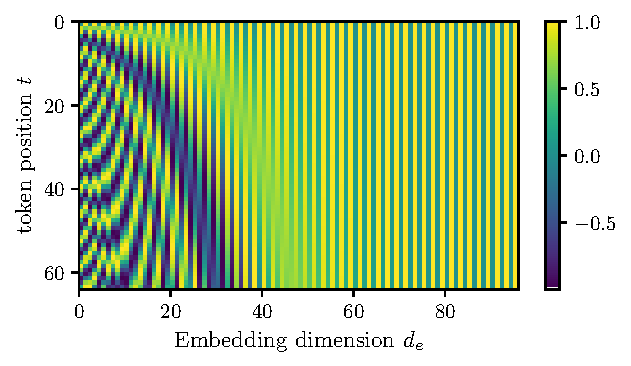
\includegraphics{positional-encoding.pdf}
  \end{center}
  \caption[Positional Encoding]{Positional Encoding. Own work.}
  \label{fig:positional-embedding}
\end{figure}

Using trigonometric functions for the positional embedding is favourable, due to being zero-centred, and resulting in values in the closed range of $[-1,1]$. These properties are long known to promote the convergence of neural networks \autocites[][8-9]{lecunEfficientBackProp2012}[][2]{ioffeBatchNormalizationAccelerating2015}.

The reason for encoding with both the sine and cosine is more subtle, as either one would suffice for absolute embeddings. \textcite[][6]{vaswaniAttentionAllYou2017} hypothesize, that besides learning the \emph{absolute} position i.e., fifth place in sequence, providing both sine and cosine also enables the model to attend to \emph{relative} positions, i.e., two places from a given token.

The positional embedding is finally added element-wisely to the token embedding to form a token's initial embedding $\gls{e}$. For the $\gls{t}$-th token of a sequence $\gls{x}$, the embedding becomes:
\begin{equation}
  \boldsymbol{e}=W_e[:, x[t]]+W_p[:, t].
  \label{eq:positional-embedding}
\end{equation}

Intuitionally, adding the positional encoding leads to a rotation of the token embedding in the embedding space. As the positional embedding is different for every location within the sequence, otherwise identical \glspl{token}, now have a unique embedding.

\subsubsection{Attention}\label{sec:attention}

\subsubsection{Position-wise Feed-Forward Networks}\label{sec:position-wise-ffn}

The attention mechanism enables tokens to attend to other inputs in the immediate context. To retain general information on the task, outside and independent of the immediate context, each Transformer block adds a point-wise \gls{feed-forward-network}, which acts as a persistent memory to the model \autocite[][3]{sukhbaatarAugmentingSelfattentionPersistent2019}.

The network consists of a linear transformation, followed by a non-linear activation function and a second linear layer. For the $l$-th layer, the \gls{MLP} is given by:

\begin{equation}
  X = X+W_{\mathrm{mlp} 2}^l \operatorname{ReLU}\left(W_{\mathrm{mlp} 1}^l X+b_{\mathrm{mlp} 1}^l 1^{\top}\right)+b_{\mathrm{mlp} 2}^l 1^{\top},
\end{equation}

with $W_{\text {mlp } 1}^l \in \mathbb{R}^{d_{\mathrm{mlp}} \times d_{\mathrm{e}}}, b_{\mathrm{mlp} 1}^l \in \mathbb{R}^{d_{\mathrm{mlp}}}, W_{\mathrm{mlp} 2}^l \in \mathbb{R}^{d_{\mathrm{e}} \times d_{\mathrm{mlp}}}$ and $b_{\mathrm{mlp} 2}^l \in \mathbb{R}^{d_{\mathrm{e}}}$ being learnable parameters identical for all \glspl{embedding} in the layer. The network is applied to each embedding separately and identically.

\textcite[][9]{vaswaniAttentionAllYou2017} set the hidden dimension to be two to eight magnitudes of the embedding dimension. The large capacity strengthens the model's ability to retain information but also contributes significantly to the high computational requirements and memory footprint of Transformers \autocites[][5]{tayEfficientTransformersSurvey2022}[][1]{kitaevReformerEfficientTransformer2020}. Both linear transformations are separated by a \gls{ReLU} \gls{activation-function} \autocite[][318]{glorotDeepSparseRectifier2011} to introduce non-linearities to the network.

Like the attention layer, the position-wise \gls{FFN} is surrounded by residual connections (see \cref{sec:residual-connections}), followed by layer normalization (see \cref{sec:layer-norm}). Both are vital for the training process and convergence of the overall network, as we show. Optionally, dropout \autocite[][1930]{srivastavaDropoutSimpleWay} is added to prevent the model from \gls{overfitting}.

\subsubsection{Residual Connections}\label{sec:residual-connections}

Recall from earlier chapters, that the encoder stacks multiple Transformer blocks, each of which consists of several sub-layers, resulting in a deep network.  While depth is required to learn hierarchical representations, the training of such a network is complicated. As neural networks are commonly trained using back-propagation, which relies on the gradient of the error to be propagated through the network starting at the last layer, vanishing or \glspl{exploding-gradient} pose a major difficulty in training deep neural nets \autocite[][1]{heDeepResidualLearning2015}. Without countermeasures, stacking multiple layers in the encoder and decoder of the Transformers impedes the gradient information to flow efficiently through the network and hampers the training behaviour \autocite[][1811]{wangLearningDeepTransformer2019}.

As a remedy, \textcite[][3]{vaswaniAttentionAllYou2017} add residual connections \autocite[][1--2]{heDeepResidualLearning2015} around each sub-layer. Like in \cref{eq:residual-connection}, the encoded token sequence $\gls{X} \in \mathbb{R}^{\gls{d}_e \times \gls{ell}_x}$ consists of the sub-layer's output added element-wisely to its input:
\begin{equation}
  \gls{X} = \gls{X} + \operatorname{sub\_layer}\left(\gls{X}\right).
  \label{eq:residual-connection}
\end{equation}

Intuitively, the residual connection provides an alternative path for information to flow through the network, since some information can bypass the sub-layer and hence reach deeper layers within the stack. Also, vanishing or \glspl{exploding-gradient} are mitigated, as gradients can bypass the sub-layer, eventually contributing towards an easier optimization \autocite[][3591]{liuRethinkingSkipConnection2020}.  Residual connections moreover help to preserve the positional embeddings (see \cref{sec:positional-encoding}), as the layer's inputs are maintained in the identity mapping. Another technique to improve the training behaviour is layer normalization.

\subsubsection{Layer Normalization}\label{sec:layer-norm}

\subsection{Transformer Networks For Tabular Data}\label{sec:tabular-transformer}

\subsubsection{TabTransformer}\label{sec:tabtransformer}

\subsubsection{FTTransformer}\label{sec:fttransformer}


\newpage
\section{Semi-Supervised Approaches (8~p)}\label{sec:semi-supervised-approaches}

\subsection{Selection of Approaches (2~p)}\label{sec:selection-of-approaches-1}

\subsection{Extensions to Gradient Boosted
  Trees (2~p)}\label{sec:extensions-to-gradient-boosted-trees}

\subsection{Extensions to TabTransformer (2~p)}\label{sec:extensions-to-tabtransformer}

\subsection{Extensions to FTTransformer (2~p)}\label{sec:extensions-to-fttransformer}


\newpage
\section{Empirical Study (19.5~p)}\label{sec:empirical-study}

\subsection{Environment (0.5~p)}\label{sec:environment}

\subsection{Data and Data Preparation (6 p)}\label{sec:data-and-data-preparation}

\subsubsection{ISE Data Set (0.5~p)}\label{sec:ise-data-set}

\subsubsection{CBOE Data Set (0.5~p)}\label{sec:cboe-data-set}

\subsubsection{Exploratory Data Analysis (2~p)}\label{sec:exploratory-data-analysis}

\subsubsection{Data Pre-Processing (1~p)}\label{sec:data-preprocessing}

\subsubsection{Feature Engineering (1.5~p)}\label{sec:feature-engineering}

\subsubsection{Train-Test Split (0.5~p)}\label{sec:train-test-split}

\subsection{Training and Tuning (10~p)}\label{sec:training-and-tuning}

\subsubsection{Training of Supervised
  Models (4~p)}\label{sec:training-of-supervised-models}


\subsubsection{Training of Semi-Supervised
  Models (4~p)}\label{sec:training-of-semi-supervised-models}


\subsubsection{Hyperparameter Tuning (2~p)}\label{sec:hyperparameter-tuning}


\subsection{Evaluation (3~p)}\label{sec:evaluation}

\subsubsection{Feature Importance
  Measure (2~p)}\label{sec:feature-importance-measure}

\subsubsection{Evaluation Metric (1~p)}\label{sec:evaluation-metric}

\newpage
\section{Results (12~p)}\label{sec:results}

\subsection{Results of Supervised
  Models (2~p)}\label{sec:results-of-supervised-models}

\subsection{Results of Semi-Supervised
  Models (2~p)}\label{sec:results-of-semi-supervised-models}

\subsection{Robustness of Results (3~p)}\label{sec:robustness-checks}

\subsection{Feature Importance (3~p)}\label{sec:feature-importance}

\subsection{Ablation Study of Models (2~p)}\label{sec:ablation-study}

\newpage
\section{Application in Transaction Cost Estimation (optional)}\label{sec:application}
\subsection{Simulation Setup (optional)}\label{sec:simulation-setup}
\subsection{Simulation Results (optional)}\label{sec:simulation-results}

\newpage
\section{Discussion (3~p)}\label{sec:discussion}

\newpage
\section{Conclusion (2~p)}\label{sec:conclusion}

\newpage
\section{Outlook (0.5~p=67.5~p)}\label{sec:outlook}

